% Pad with two zeroes
\newcommand\padzeroes[1]{\ifnum #1 < 10 0\fi\ifnum #1 < 100 0\fi #1}

% This stuff does automatic user story numbering
\newcommand{\ustorylbl}{FREQ}
\newcounter{storynr}
\newcommand{\story}{\subsubsection{\ustorylbl-\padzeroes{\arabic{storynr}}}}
\stepcounter{storynr}

\section{Eisen}
\subsection{Use Case Diagram}
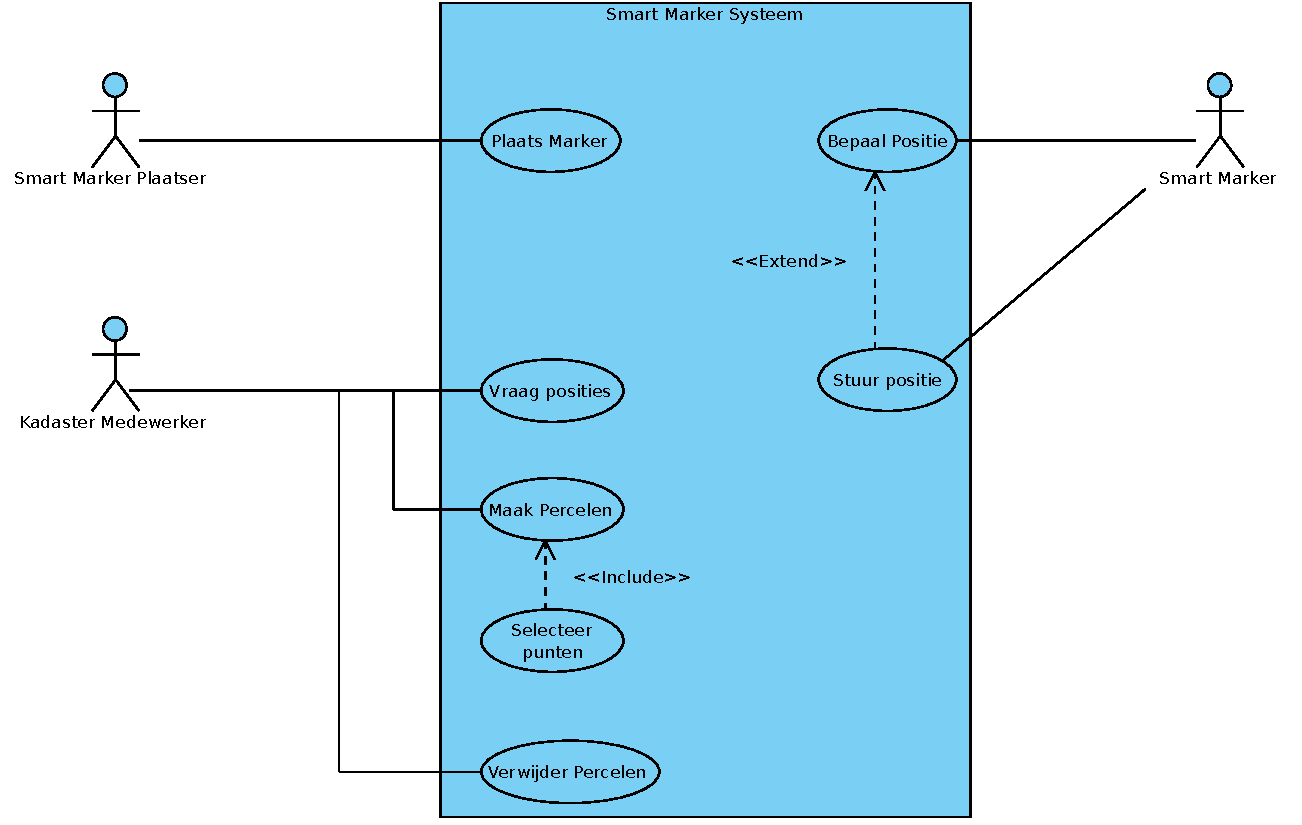
\includegraphics[width=\textwidth]{functional/use_case.pdf}

\subsection{User Stories}
\story
Als Kadaster medewerker wil ik de locatie van de Smart Markers kunnen zien op
een kaart.
\stepcounter{storynr}

\story
Als Kadaster medewerker wil ik de Smart Markers kunnen identificeren.
\stepcounter{storynr}

\story
Als Kadaster medewerker wil ik een kadastrale registratie kunnen doen,
met behulp van de Smart Markers kaart.
\stepcounter{storynr}

\story
Als Smart Marker plaatser wil ik kunnen zien dat een Smart Marker aanstaat.
\stepcounter{storynr}

\story
Als Smart Marker plaatser wil ik kunnen zien dat een Smart Marker verbonden
is met het netwerk.
\stepcounter{storynr}

\story
Als Smart Marker plaatser wil ik geen systeeminstellingen hoeven aan te passen.
\stepcounter{storynr}

\story
Als Smart Marker plaatser wil ik weinig onderhoud hoeven te doen aan de
Smart Marker (batterijduur).
\stepcounter{storynr}

\story
Als Kadaster medewerker wil ik een kaart zien waarop alle meetpunten aangegeven zijn.
\stepcounter{storynr}

\story
Als Kadaster medewerker wil ik de informatie van een meetpunt/perceel op de kaart kunnen inzien.
\stepcounter{storynr}

\story
Als Kadaster medewerker wil ik van meerdere meetpunten samen een perceel kunnen maken.
\stepcounter{storynr}

\story
Als Kadaster medewerker wil ik een gemaakt perceel kunnen verwijderen.
\stepcounter{storynr}

\newpage
\subsection{Milestones}
\begin{itemize}
    \item Een prototype welke testdata naar een gateway kan versturen
    \item Een Smart Marker welke zijn positie kan bepalen en deze door kan sturen
    \item Een weergave van de meetpunten op de kaart tonen
\end{itemize}
\subsection{Definition of Done}
Iets is pas klaar als:
\begin{itemize}
    \item De code geschreven is volgens de codestandaard die in het plan
          van aanpak beschreven is\
    \item De code volledig is getest volgens ons testplan
    \item De code ook unittests heeft waar het nodig is
    \item De documentatie klopt met de code
    \item De code is gereviewd door tenminste één teamgenoot
\end{itemize}
